\documentclass[11pt,a4paper, margin=1in]{article}
\usepackage{fullpage}
\usepackage{amsfonts, amsmath, pifont}
\usepackage{amsthm}
\usepackage{graphicx}
\usepackage{float}

\usepackage{tkz-euclide}
\usepackage{tikz}
\usepackage{pgfplots}
\pgfplotsset{compat=1.13}

\usepackage{geometry}
 \geometry{
 a4paper,
 total={210mm,297mm},
 left=10mm,
 right=10mm,
 top=10mm,
 bottom=20mm,
 }

 \author{
  Karaçanta, Kaan\\
  \texttt{e244854@metu.edu.tr}
}

\newcommand{\mySin}[1]{\textstyle\sin\left(#1\right)}
\newcommand{\myCos}[1]{\textstyle\cos\left(#1\right)}
\usepackage{hyperref}

\usepackage{inconsolata}
\usepackage{listings}
\usepackage{xcolor}
\usepackage[utf8]{inputenc}
\usepackage[T1]{fontenc}

\definecolor{codegreen}{rgb}{0,0.6,0}
\definecolor{codegray}{rgb}{0.5,0.5,0.5}
\definecolor{codepurple}{rgb}{0.58,0,0.82}
\definecolor{backcolour}{rgb}{0.95,0.95,0.92}

\lstdefinestyle{mystyle}{
    backgroundcolor=\color{backcolour},
    commentstyle=\color{codegreen},
    keywordstyle=\color{magenta},
    numberstyle=\tiny\color{codegray},
    stringstyle=\color{codepurple},
    basicstyle=\ttfamily\footnotesize,
    breakatwhitespace=false,
    breaklines=true,
    captionpos=b,
    keepspaces=true,
    numbers=left,
    numbersep=5pt,
    showspaces=false,
    showstringspaces=false,
    showtabs=false,
    tabsize=2
}

\lstset{style=myStyle}

\title{CENG 371 - Scientific Computing \\
Fall' 2024 - 2025 \\
Homework 1}

\begin{document}
\maketitle

\noindent\rule{19cm}{1.2pt}

% f(x) = (x * (((x+1)/x) - 1)) - 1
\section*{Question 1}

\begin{enumerate}
    % the plot of the function
    \item The plot of the function \( g(n) = f(n) / \epsilon \) is given below, where \( \epsilon = 10^{-6} \).
    \begin{figure}[H]
        \centering
        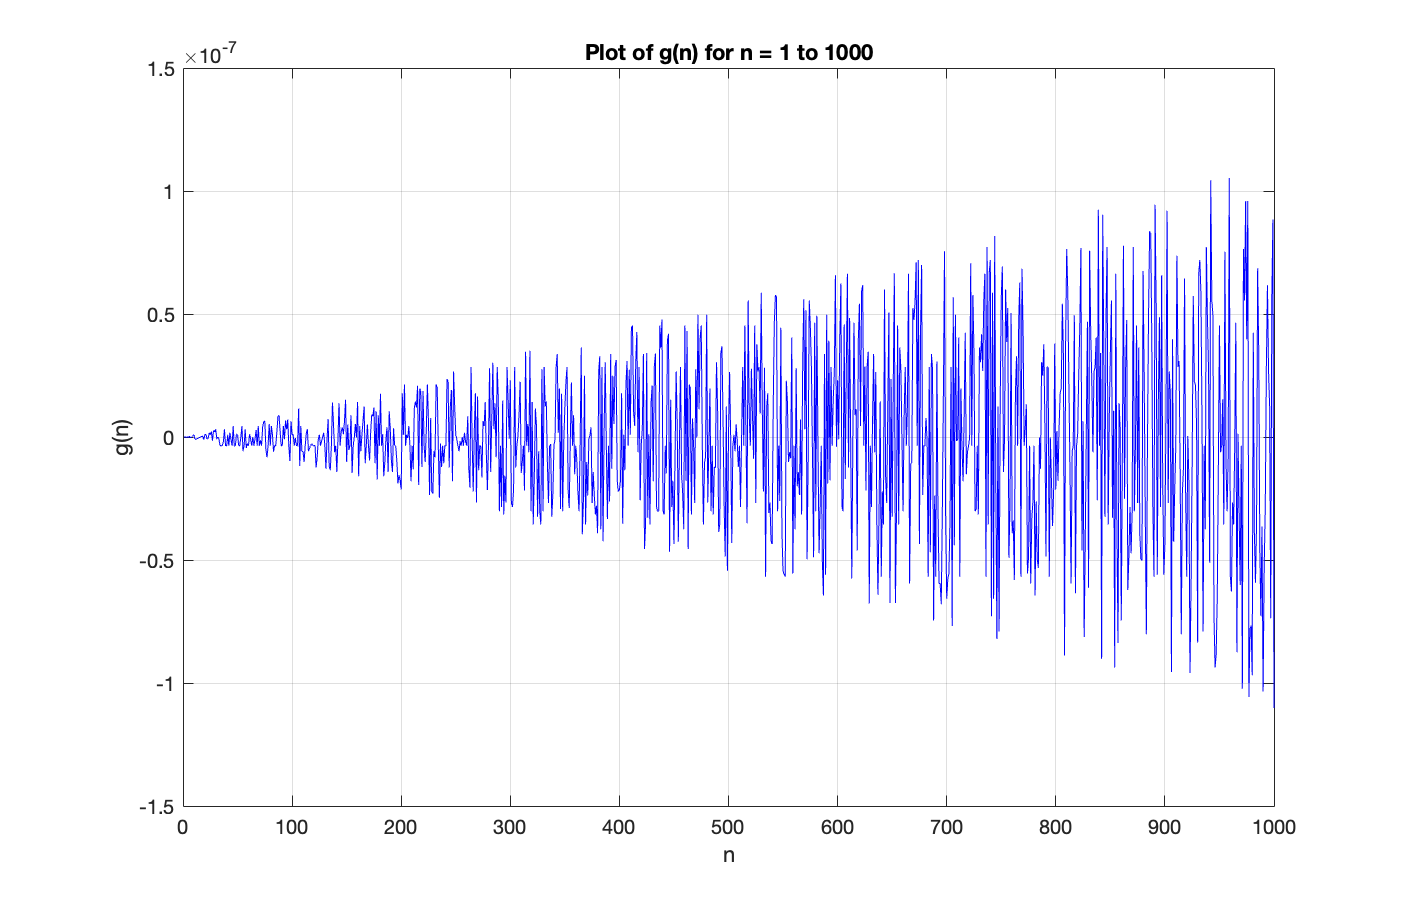
\includegraphics[width=0.9\textwidth]{q1.png}
        \caption{The plot of \(g(n)\)}
    \end{figure}

    % Which of the values of n satisfy g(n) = 0?
    \item The values of n where \( g(n) = 0 \) are \( 1, 2, 4, 8, 16, 32, 64, 128, 256, 512 \). In other words, \( g(n) = 0 \) when \(n\) is a power of 2. 
    
    % Explain why g(n) ̸= 0 of majority of n.
    \item For the majority of values of \( n \), we have \( g(n) \neq 0 \) due to the structure of the function \( g(n) = \frac{f(n)}{\epsilon} \), where \( f(x) = x\left(\frac{x+1}{x} - 1\right) - 1 \), although it is mathematically \(0\) for all integers in that range.

    \begin{itemize}
        \item \textbf{Function Form:} The function \( f(x) \) involves both subtraction and division within its expression. Due to the presence of rational numbers and integer operations in computers, the function rarely yields an exact zero result. Since \( \epsilon \) is a divisor, \( g(n) \) will only be zero when exactly \( f(n) = 0 \), which does not happen for integer values of \( n \) other than the powers of 2.
        \item \textbf{Non-Zero Outcomes:} For integer values of \( n \), it is unlikely for \( f(n) \) to balance out to exactly zero due to the continuous fractions or decimal components in the calculation, especially when using floating-point arithmetic, in division, small precision errors accumulate, resulting in values that are not exactly zero. As a result, for most \( n \), \( g(n) \) does not reach exactly zero.
    \end{itemize}

    In summary, the structure of \( f(x) \) results in values that rarely lead to \( f(n) = 0 \) in computers due to rounding errors and their accumulations, so \( g(n) \neq 0 \) for the majority of \( n \).
    
    % g(n) seems to grow in size. Why?
    \item The values of \( g(n) \) appear to grow in size as \( n \) increases, not due to mathematical growth, but due to computational problems. 
    As \( n \) grows, the floating-point operations involved in calculating \( f(n) \) lead to small discrepancies from zero, and when you do these operations with bigger integers, the errors become larger, and even more visible when amplified with \(\epsilon\).

\end{enumerate}

% Generate an array of numbers k where ki = 1 + (e+6 + 1 - ni) * e-8 ni = 1, 2, ..., e+6
\section*{Question 2}

\begin{enumerate}

    % Calculate the theoretical result for the sum of the element of k.
    \item Each element \( k_i \) is defined by the formula:
    \[
    k_i = 1 + (10^6 + 1 - n_i) \times 10^{-8}
    \]
    where \( n_i \in [1, 10^6] \).
    
    The theoretical sum of all elements in \( k \) can be calculated as:
    \[
    \text{Theoretical Sum} = 10^6 + \left(10^6 \times \frac{10^6 + 1}{2} \times 10^{-8}\right)
    \]
    
    This sum consists of \( 10^6 \) terms of 1 plus the sum of a sequence of terms that scale with \( 10^{-8} \). Thus, the theoretical sum is \( 10^6 + 5000.005 \).

    % In no more than two sentences, explain the idea of pairwise summation
    \item Pairwise summation is an algorithm that reduces accumulated rounding errors by summing pairs of elements in a sequence, instead of summing sequentially. It divides the array into pairs, sums each pair, and then sums the resulting sums recursively.

    % Calculate the sum of the elements of k using naive summation, compensated summation, and pairwise summation in single and double precisions.
    \item These sums can be seen in the picture below, as my Matlab code's output. The results are as follows:
    \begin{figure}[H]
        \centering
        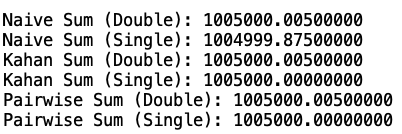
\includegraphics[width=0.5\textwidth]{q2_1.png}
        \caption{The sum of the elements of \( k \) using different summation methods}
    \end{figure}

    % Compare the methods’ errors and runtimes.
    \item Full comparison of the methods' results, errors and runtimes are as follows:
    \begin{figure}[H]
        \centering
        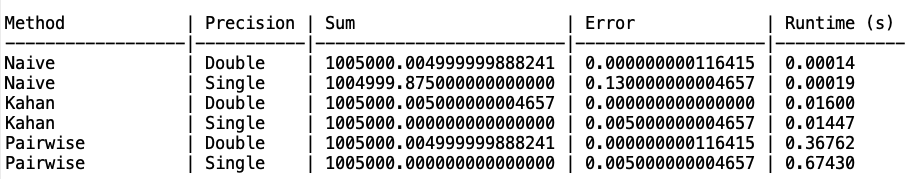
\includegraphics[width=0.9\textwidth]{q2_2.png}
        \caption{Comparison of the methods' results, errors and runtimes}
    \end{figure}

    % Comment on your results. As a suggestion, you can comment on the differences, possible improvements, etc.
    \item The results show that both Kahan and pairwise summation techniques improve accuracy by reducing rounding errors. While naive summation is the simplest and fastest method, it suffers from significant numerical errors in single precision, especially for large arrays due to the accumulation of rounding errors. Kahan summation provides a reliable way to compensate for rounding errors but is slower than naive summation. Pairwise summation performs well in both single and double precision and typically provides results close to those of Kahan summation. While being effective at reducing errors, it has a variable runtime, and Kahan outperfomed it in both precisions and runtimes in this case. 
    
    To further improve accuracy and efficiency in summation, several approaches can be considered, other than increasing the precision of course. One option is parallelizing pairwise summation, the others can be as well, can enhance performance on multi-core systems by concurrently executing recursive sums. Additionally, a hybrid method that combines Kahan and pairwise summation could capture more precise results by balancing accuracy and runtime. Finally, adaptive algorithms that select, or just selecting manually, the optimal summation technique based on input characteristics may also yield improvements, but even if this kind of selection is possible, it would be computationally expensive and hard to implement, so it might be used in very specific cases maybe.
    
    In summary, Kahan summation is preferable for applications where accuracy is critical, while pairwise summation can be useful when an alternative error reduction method is needed. The choice between single and double precision also affects accuracy, with double precision generally yielding more reliable results, as expected, at the cost of increased memory usage.

\end{enumerate}

\end{document}